%%%%%%%%%%%%%%%%%%%%%%%%%%%%%%%%%%%%%%%%%
% Jacobs Landscape Poster
% LaTeX Template
% Version 1.1 (14/06/14)
%
% Created by:
% Computational Physics and Biophysics Group, Jacobs University
% https://teamwork.jacobs-university.de:8443/confluence/display/CoPandBiG/LaTeX+Poster
% 
% Further modified by:
% Nathaniel Johnston (nathaniel@njohnston.ca)
%
% This template has been downloaded from:
% http://www.LaTeXTemplates.com
%
% License:
% CC BY-NC-SA 3.0 (http://creativecommons.org/licenses/by-nc-sa/3.0/)
%
%%%%%%%%%%%%%%%%%%%%%%%%%%%%%%%%%%%%%%%%%

%----------------------------------------------------------------------------------------
%	PACKAGES AND OTHER DOCUMENT CONFIGURATIONS
%----------------------------------------------------------------------------------------

\documentclass[final]{beamer}

\usepackage[scale=1.24]{beamerposter} % Use the beamerposter package for laying out the poster

\usetheme{confposter} % Use the confposter theme supplied with this template

\setbeamercolor{block title}{fg=ngreen,bg=white} % Colors of the block titles
\setbeamercolor{block body}{fg=black,bg=white} % Colors of the body of blocks
\setbeamercolor{block alerted title}{fg=white,bg=dblue!70} % Colors of the highlighted block titles
\setbeamercolor{block alerted body}{fg=black,bg=dblue!10} % Colors of the body of highlighted blocks
% Many more colors are available for use in beamerthemeconfposter.sty

%-----------------------------------------------------------
% Define the column widths and overall poster size
% To set effective sepwid, onecolwid and twocolwid values, first choose how many columns you want and how much separation you want between columns
% In this template, the separation width chosen is 0.024 of the paper width and a 4-column layout
% onecolwid should therefore be (1-(# of columns+1)*sepwid)/# of columns e.g. (1-(4+1)*0.024)/4 = 0.22
% Set twocolwid to be (2*onecolwid)+sepwid = 0.464
% Set threecolwid to be (3*onecolwid)+2*sepwid = 0.708

\newlength{\sepwid}
\newlength{\onecolwid}
\newlength{\twocolwid}
\newlength{\threecolwid}
\setlength{\paperwidth}{48in} % A0 width: 46.8in
\setlength{\paperheight}{36in} % A0 height: 33.1in
\setlength{\sepwid}{0.024\paperwidth} % Separation width (white space) between columns
\setlength{\onecolwid}{0.22\paperwidth} % Width of one column
\setlength{\twocolwid}{0.464\paperwidth} % Width of two columns
\setlength{\threecolwid}{0.708\paperwidth} % Width of three columns
\setlength{\topmargin}{-0.5in} % Reduce the top margin size
%-----------------------------------------------------------

\usepackage{graphicx}  % Required for including images

\usepackage{booktabs} % Top and bottom rules for tables

%----------------------------------------------------------------------------------------
%	TITLE SECTION 
%----------------------------------------------------------------------------------------

\title{Text Analysis of News Articles \\
(Building a Protest Dataset through Machine Learning) } % Poster title

\author{Howard Liu (\textcolor{blue}{hao.liu@duke.edu}) Sophie Lee (\textcolor{blue}{sophie.lee@duke.edu}), \& Haohan Chen (\textcolor{blue}{haohan.chen@duke.edu})} % Author(s)

\institute{Department of Political Science, Duke University} % Institution(s)

%----------------------------------------------------------------------------------------

\begin{document}

\addtobeamertemplate{block end}{}{\vspace*{2ex}} % White space under blocks
\addtobeamertemplate{block alerted end}{}{\vspace*{2ex}} % White space under highlighted (alert) blocks

\setlength{\belowcaptionskip}{2ex} % White space under figures
\setlength\belowdisplayshortskip{2ex} % White space under equations

\begin{frame}[t] % The whole poster is enclosed in one beamer frame

\begin{columns}[t] % The whole poster consists of two major columns, the second of which is split into three columns  - the [t] option aligns each column's content to the top

\begin{column}{\sepwid}\end{column} % Empty spacer column

\begin{column}{\onecolwid} % The first column

%----------------------------------------------------------------------------------------
%	OBJECTIVES
%----------------------------------------------------------------------------------------

\begin{alertblock}{Objectives}

In this project, we attempt to build a dataset of political conflict. We aim to extract important information with machine learning algorithm from news reports of political conflicts. Specifically, our methods automatically code entries of news on: \textit{where} the conflicts happen; \textit{who} are involved, and; \textit{what} type of issues are at stake. \\

We attempt to improve on the \textit{state-of-art} of the political science scholarship by tackling the following challenges:
\begin{itemize}
	\item Separating multiple events in one news report
	\item Machine-coding actors involved in conflicts
	\item Machine-coding types of issues at stake 
\end{itemize}

\end{alertblock}

%----------------------------------------------------------------------------------------
%	INTRODUCTION
%----------------------------------------------------------------------------------------

\begin{block}{Introduction}

\noindent Building a reliable data is crucial in political science as political scientists study phenomena involving human interactions that are not always clean-cut. Although domestic protest is one of the central interest of peace and security research, building a comprehensive data that encompass all countries is extremely difficult due to challenges non-democratic regimes pose on researchers collecting data. Hence, analyzing news articles has become a new way of studying many aspects in such societies, yet handling massive texts and producing a dataset has still room for improvement. One existing data, that is widely used in the field is World-Wide Integrated Crisis Early Warning System (W-ICEWS)\cite{icews}, yet the data suffer from the following three problems.\\
\vspace{1cm}
\noindent {\bf First,} ICEWS does not account for news articles that contain more than one events. \\
\noindent {\bf Second,} ICEWS does not differentiate location identifiers that refer to the location of news agencies and the location of the events.\\
\noindent {\bf Third,} ICEWS does not code the event type.

\noindent Hence, we aim to resolve these issues and improve the accuracy of the current ICEWS data. \\
\end{block}

%------------------------------------------------

%\begin{figure}
%
\includegraphics[width=0.8\linewidth]{placeholder.jpg}
%\caption{Figure caption}
%\end{figure}

%----------------------------------------------------------------------------------------

\end{column} % End of the first column

\begin{column}{\sepwid}\end{column} % Empty spacer column

\begin{column}{\threecolwid} % Begin a column which is three columns wide (column 2)

\begin{columns}[t,totalwidth=\twocolwid] % Split up the three columns wide column

\begin{column}{\onecolwid}\vspace{-.6in} % The first column within column 2 (column 2.1)

%----------------------------------------------------------------------------------------
%	DATA
%----------------------------------------------------------------------------------------

\begin{block}{Data}

We train and test our model with a subset of ICEWS data containing 642 English news reports from 2001 to 2014 on protests in China. Variables include:

\begin{itemize}
\item Original text of the report
\item Human-coded location
\item Human-coded issue types
\end{itemize}

For the the coding of location and actors, we fitted the model with the full dataset. For issue types, 80\% of the cases were used as the training set and the rest as the test set.

\end{block}

%----------------------------------------------------------------------------------------

\end{column} % End of column 2.1.1

\begin{column}{\sepwid}\end{column} % Empty spacer column

\begin{column}{\twocolwid}\vspace{-.6in} % The second column within column 2 (column 2.1.2)

%----------------------------------------------------------------------------------------
%	conflict map
%----------------------------------------------------------------------------------------

\begin{block}{Frequency of Protests in Each Chinese Province (2001-2014)}
\begin{figure}
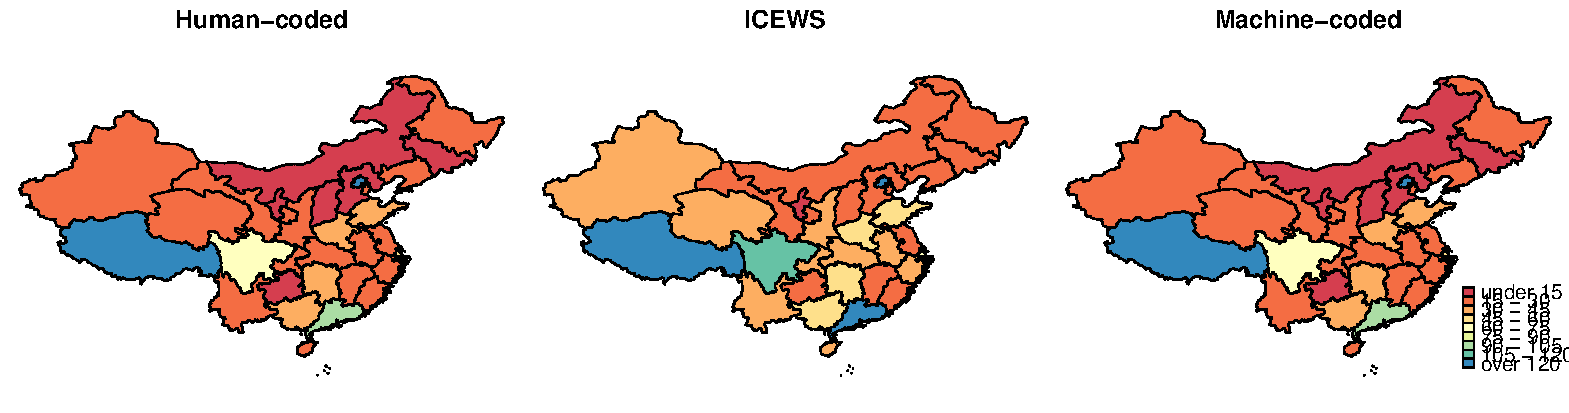
\includegraphics[width=0.8\linewidth]{china_maps.pdf}
\caption{Figure caption}
\end{figure}
\end{block}

\end{column} % End of column 2.1.2
\end{columns} % End of the split of column 2 - any content after this will now take up 2 columns width

%----------------------------------------------------------------------------------------
%	IMPORTANT RESULTs   (column 2.2.1)
%----------------------------------------------------------------------------------------
\vspace{10mm}

\begin{columns}[t,totalwidth=\threecolwid] % Split up the two columns wide column

\begin{column}{\twocolwid}\vspace{-.6in} % The second column within column 2 (column 2.2)

\begin{alertblock}{Important Results}
\begin{itemize}
\item Locations are coded correctly for 66\% of the cases, which is substantially higher than the current ICEWS data, of which accuracy rate is 47\%.
\item We were able to code actors and issue types as well, yet (1) we do not have a manually coded variable for the former and hence unable to compute the accuracy rate, and (2) the performance of the latter still needs to be improved greatly.
\end{itemize}

\end{alertblock} 

\end{column}


%----------------------------------------------------------------------------------------
%	Concluding remarks (2.2.2)
%----------------------------------------------------------------------------------------
\begin{column}{\sepwid}\end{column} % Empty spacer column


\begin{column}{\onecolwid}\vspace{-.6in} % The second column within column 2 (column 2.2.2)


\begin{block}{Concluding Remarks}
\begin{itemize}
\item The machine-coding methods we develop outperform the \textit{state-of-art} in geo-coding. 
\item Our methods have potential to code and classify events on more characters that previously rely on human coding.
\end{itemize}


\end{block}

\end{column}
\end{columns}


%\begin{columns}[t,totalwidth=\threecolwid] % Split up the two columns wide column again

%----------------------------------------------------------------------------------------
%	Methods
%----------------------------------------------------------------------------------------
\begin{columns}[t,totalwidth=\threecolwid] % Split up the three columns wide column

\begin{column}{\onecolwid} % The first column within column 2 (column 2.3.1)



\begin{block}{Methods}
We first identified the news sources that contaminate the data and removed lines that are not part of the news articles. We then used a dictionary of provinces and search for province names. Based on the number of provinces in one article, we analyzed the text using the Latent Dirichlet Allocation (LDA) method, setting the number of topics equal to the number of provinces produced. Then, we examined the most frequent words of each topic and searched for actor types.\\

To code issue types, we first created the document term matrix. We then used the human-coded issue type as the outcome and fit the dtm into SVM, Bagging, Boosting, Random Forest, and Trees. We compared the performance and examined consensus rates of each model. \cite{jurka2011rtexttools}.


\end{block}
\end{column} % End of column 2.3.1

\begin{column}{\sepwid}\end{column} % Empty spacer column
%----------------------------------------------------------------------------------------
%	Performance
%----------------------------------------------------------------------------------------
\begin{column}{\onecolwid} % The second column within column 2 (column 2.2)

\begin{block}{Performance}

The performance substantially improve upon existing methods in geo-coding conflict events. Nevertheless, our attempt on actor and event type coding, albeit its originality, has less-than-ideal performance. We report the accuracy rate of matching coding, using human coding and ICEWS data as benchmarks.

\vspace{1cm}

\begin{table}[!H]
\centering
\begin{tabular}{l|ccc}
\hline\hline
Data&Manual & ICEWS & Ours\\
\hline
Location&100\% & 47\% & 66\%\\
Actors& missing & 100\%  & 3\%\\
\hline\hline
\end{tabular}
\caption{Accuracy rates: Location and Actors}
\label{tab:accuracy}
\end{table}

\vspace{1cm}

\begin{table}[!H]
\centering
\begin{tabular}{l|ccc}
\hline\hline
Model& Precision & Recall & F-Score\\
\hline
SVM& .0267 & .111 & .043 \\
Boosting& .067 & .072 & .064 \\
Bagging& .129 & .121 & .104 \\
Random Forest& .043 & .068 & .044 \\
Tree& .104 & .088 & .081 \\
\hline\hline
\end{tabular}
\caption{Accuracy rates: Issue Type}
\label{tab:svm}
\end{table}

\end{block}

%----------------------------------------------------------------------------------------

\end{column} % End of column 2.3.2

\begin{column}{\sepwid}\end{column} % Empty spacer column


%----------------------------------------------------------------------------------------
%	CONCLUSION
%----------------------------------------------------------------------------------------

%\begin{block}{Conflict Map: Machine}
%\begin{figure}
%
\includegraphics[width=0.8\linewidth]{placeholder.jpg}
%\caption{Figure caption}
%\end{figure}
%\end{block}

\begin{column}{\onecolwid} % The third column



\begin{block}{Limitation and Future Works}

\begin{itemize}
\item The training set is small, thus plan to expand it.
\item The performance of actors and issue types need much improvement. We plan to further examine the sparsity of DTM, classification model, and pre-processing with post-tagging.
\end{itemize}

\end{block}

%----------------------------------------------------------------------------------------
%	REFERENCES
%----------------------------------------------------------------------------------------

\begin{block}{References}
\begin{thebibliography}{2}
\bibitem{icews} Martin, Lockheed. 2014. Integrated Crisis Early Warning System (ICEWS).
\bibitem{jurka2011rtexttools} Jurka, Timothy P and Collingwood, Loren and Boydstun, Amber E and Grossman, Emiliano and Others. 2011. Rtexttools: A supervised learning package for text classification

\end{thebibliography}

%\nocite{*} 
%\small{\bibliographystyle{unsrt}
%\bibliography{sample}\vspace{0.75in}}

\end{block}

%----------------------------------------------------------------------------------------
%	ACKNOWLEDGEMENTS
%----------------------------------------------------------------------------------------

%\setbeamercolor{block title}{fg=red,bg=white} % Change the block title color

%\begin{block}{Acknowledgements}

%\small{\rmfamily{Nam mollis tristique neque eu luctus. Suspendisse rutrum congue nisi sed convallis. Aenean id neque dolor. Pellentesque habitant morbi tristique senectus et netus et malesuada fames ac turpis egestas.}} \\

%\end{block}

%----------------------------------------------------------------------------------------
%	CONTACT INFORMATION
%----------------------------------------------------------------------------------------

%\setbeamercolor{block alerted title}{fg=black,bg=norange} % Change the alert block title colors
%\setbeamercolor{block alerted body}{fg=black,bg=white} % Change the alert block body colors

%\begin{alertblock}{Contact Information}
%\centering
%Howard Liu \\
%\href{mailto:hao.liu@duke.edu}{hao.liu@duke.edu}

%\end{alertblock}

\end{column} % End of the third column

%----------------------------------------------------------------------------------------



\end{columns} % End of the three columns in column 2.3
\end{column} % End of the second column that encompass three columns
\end{columns} % End of all the columns in the poster
\end{frame} % End of the enclosing frame

\end{document}
